\documentclass{article}
\usepackage[utf8]{inputenc}
\usepackage{graphicx}
\usepackage{float}
\usepackage{epsfig}
\usepackage{blindtext}
\usepackage{graphicx}
\usepackage[T1]{fontenc}
\usepackage{amsmath}

\title{MATH 444 PS4}
\author{Connor Wolfe}
\date{April 2017}
\begin{document}
\maketitle

\section*{Problem 1}
\subsection*{Introduction}
This problem asks us to run a PCA classifier on the handwritten digits data set.  We will explore the optimal number of principal components to model the data with by running the algorithm with m=5, 10... 80 principal components.  We will then test the success of classifier on the training set and on the test set.  
\\
In order to determine the success frequency of the classifier we will divide the number of correctly classified points by the total number of points as follows from line 32 of Q1.mat
\begin{verbatim}
            success_rate_test=num_correct_test/size(I_test,2);
\end{verbatim}

\subsection*{PCA Classifier Algorithm}
The PCA Classifier is supervised learning classification algorithm.  Using a training set with data points and annotations, it will classify a new data point by projecting it in the direction of every cluster and see which best classifies the data.  The algorithm is run in three steps: partition the training data by cluster, form projectors of every cluster, and find which projector best classifies a new point.
\\We calculate the projector of every cluster in line 29 of the PCA.mat function as follows: 
\begin{verbatim}
        P{i}=u{i}(:, 1:m) * u{i}(:, 1:m)'
\end{verbatim}

\\In order to classify a new point x, we will calculate the frobenius norm of the x's projection onto the subspace of each cluster P{k}.  We calculate this as follows:
\begin{verbatim}
        norms(k)=norm(P{k}*X(:,i), 'fro');
\end{verbatim}
We then find which cluster best classifies x by seeing which frobenius norm is maximum. 

\subsection*{Data}
\begin{figure}[H]
    \centerline
    {
    \includegraphics[width=15cm, height=6.5cm]{Q1_test}
    }
    \caption{\label{fig:my figure} Frequency of successful classification using a PCA classifier and 'HandwrittenDigits.mat' as the training set and 'HandwrittenDigitsTestset.mat' as the test set.  Note the frequency improves as the number of principal components approaches 15 and then declines}
\end{figure}

\begin{figure}[H]
    \centerline
    {
    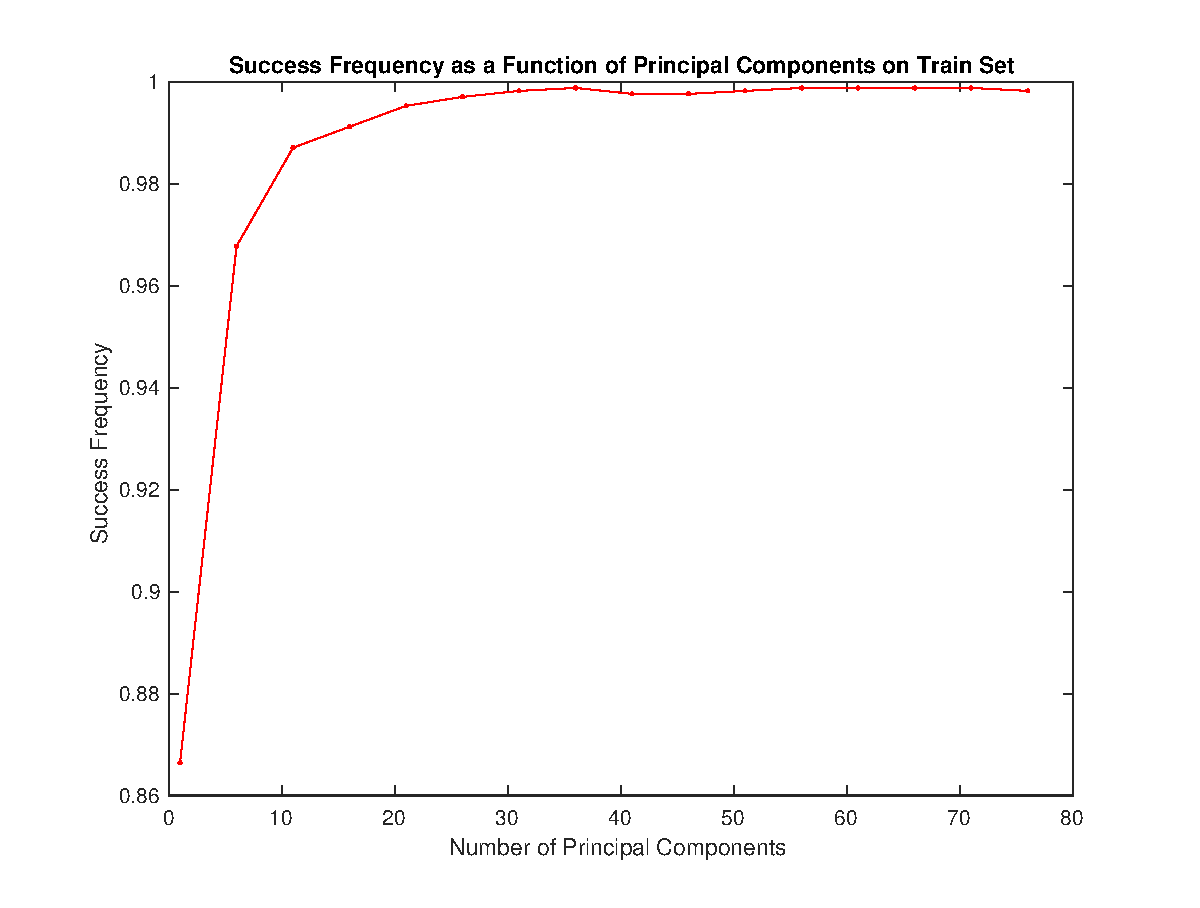
\includegraphics[width=15cm, height=6.5cm]{Q1_train}
    }
    \caption{\label{fig:my figure} Frequency of successful classification using a PCA classifier and 'HandwrittenDigits.mat' as both the training set and test set.  Note the frequency improves as a function of the number of principal components }
\end{figure}

\subsection*{Analysis}
We can see that the PCA Classifier was generally highly effective, correctly classifying consistently over 90\% of data points.  Note that in figure 1 when we test with a different set than we trained with, the success frequency does not increase as the number of principal components increases.  Instead, we want to project onto an optimal number of principal components of roughly 15.  It makes sense that we do not want the subspace of each cluster to be spanned by too small a number of principal components  because then we underfit and do not capture the entirety of a cluster, just the center.  And it makes sense that we do not want the subspace of the cluster to be spanned by too large a number of principal components because then we overfit and every point becomes an entire subspace, so no two points are classified together.  This figure shows that the optimal number of principal components is roughly 15.
\\We notice though that in figure 2, when the test set and training set are the same, that as the number of principal components increases, so too does the success frequency. This makes sense though, because we are overfitting points to themselves. When m = the dimensions of each point, we will note a 100\% success frequency as every point will be projected onto itself by its clusters projector.  

\section*{Problem 2}
\subsection*{Introduction}
This problem asks us to analyze the same handwritten digits data, but now using the k-nearest neighbor algorithm.  We will run the algorithm with varying values of k to determine which yields the highest success rate.  

\subsection*{K-Nearest Neighbor Algorithm}
This is another supervised learning algorithm which classifies each data point x by how close it is to values in the training set.  It runs in two steps: it finds the k nearest vectors in the training set to x and then it classifies x to whichever cluster is most densely represented.  We calculate the distance of x to each point in the training set on line 11 of KNN.mat as follows:
\begin{verbatim}
           dist(j)=sqrt(sum((X_{train}(:,j)- x_{cur}).^2));

\end{verbatim}
We then sort the dist matrix and create a new vector k\_nearest which stores the indices of the closest k elements.  In order to see which cluster is majority we find the mode as follows on line 16: 
\begin{verbatim}
    I_knn(i)=mode(k_nearest);
\end{verbatim}

I\_knn thus stores the cluster that k-nearest neighbor classifies each point in the test set. Note that we find the majority using the mode function, so if two clusters are equally represented, the cluster which appears first in the k\_nearest vector will be used. 

\subsection*{Data}
\begin{figure}[H]
    \centerline
    {
    \includegraphics[width=15cm, height=6.5cm]{Q2_plot}
    }
    \caption{\label{fig:my figure} Frequency of successful classification using a k-nearest neighbor classifier, 'HandwrittenDigits.mat' as the training set and 'HandwrittenDigitsTestset.mat' as the test set.  Note the frequency declines as k increases}
\end{figure}

\subsection*{Analysis}
Again we see a successful classifier, as we correctly classify over 80\% of points, and over 90\% when k is small enough.  Note that if we had tested with the training set and only analyzed k=1 neighbor, we would have 100\% success because we the first nearest neighbor of every x in the test set would be its analogue in the training set, so it would always classify properly.

\section*{Problem 3}
\subsection*{Introduction}
This problem asks us to analyze a new file 'ForestSpectra.mat' which contains data corresponding to 4 types of forest: birch, fir, pine, and shrub.   We also have their annotation.  We will analyze this data using an LDA classifier.  Furst we will find the first 4 LDA directions and show plots of how the data clusters.  Then we will use the LDA directions to classify data from the 'ForestSpectraTest.mat' file.  

\subsection*{LDA Classifier}
An LDA classifier is another projection classifier which uses the LDA instead of PCA to find the projection direction. This algorithm runs in three steps: first we calculate the LDA components of every cluster in the training set.  Then we calculate their centroids.  And lastly we see which projector best classifies each incoming point x. 
\\First we compute the LDA following the 'LDA.mat' function from PS3 as follows:
\begin{verbatim}
    [V,D]= LDA(X_train, I_train, 1);
\end{verbatim}
Next we calculate Z, the projections of X along the eigenvectors, for every cluster as follows:
\begin{verbatim}
        Z{i}=V'*X_train(:,I_train==(i));
\end{verbatim}
For each Z, we compute its centroid:
\begin{verbatim}
        c{i}=(1/size(Z{i},2)) * sum(Z{i},2);
\end{verbatim}
And then we classify each point x by storing the frobenius norm of its projection along each cluster's LDA directions and its centroid:
\begin{verbatim}
        norms(i)=norm(Q*x - c{i}, 'fro');
\end{verbatim}
Whichever cluster minimizes the norms matrix is the appropriate cluster for point x.


\subsection*{Data}
\begin{figure}[H]
    \centerline
    {
    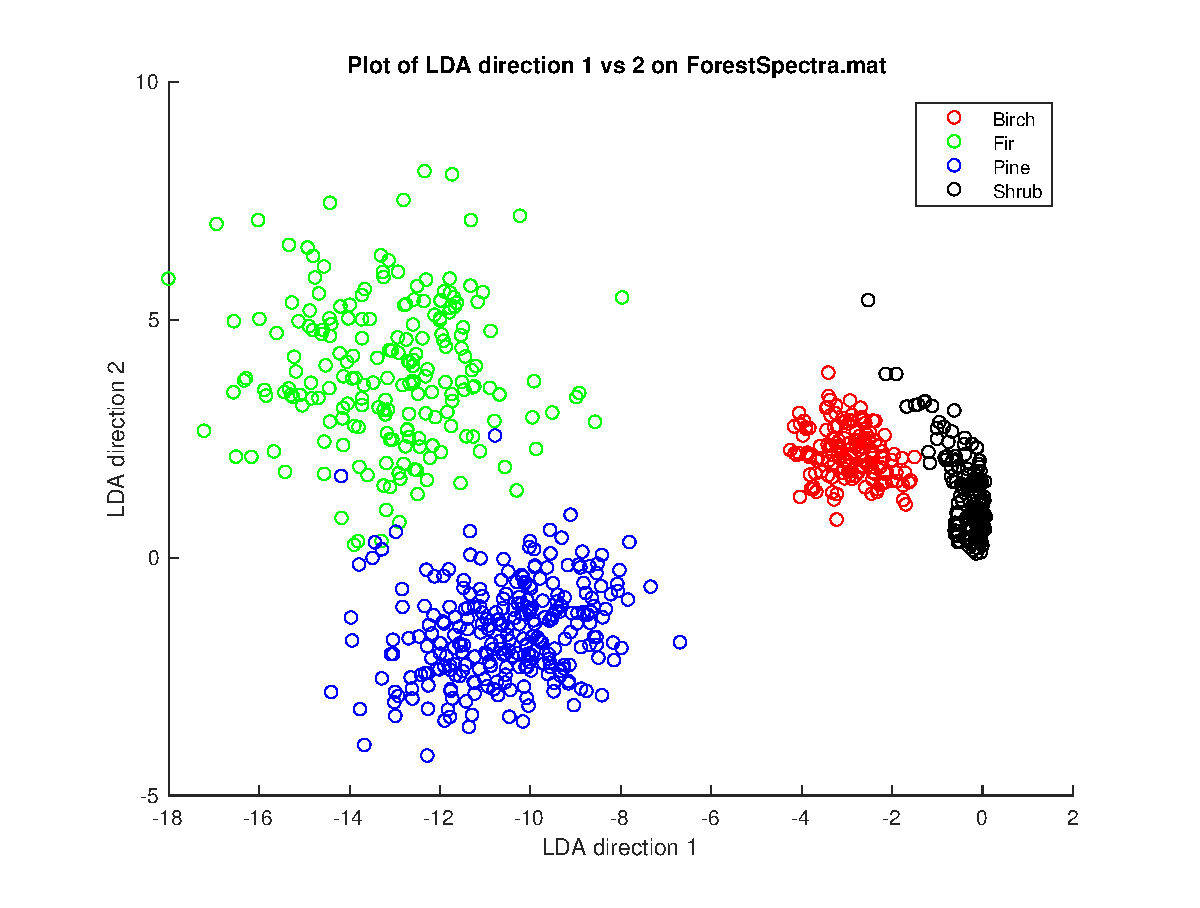
\includegraphics[width=15cm, height=6.5cm]{Q3_2directions}
    }
    \caption{\label{fig:my figure} LDA Clustering of 'ForestSpectra.mat' along first 2 LDA directions }
\end{figure}

\begin{figure}[H]
    \centerline
    {
    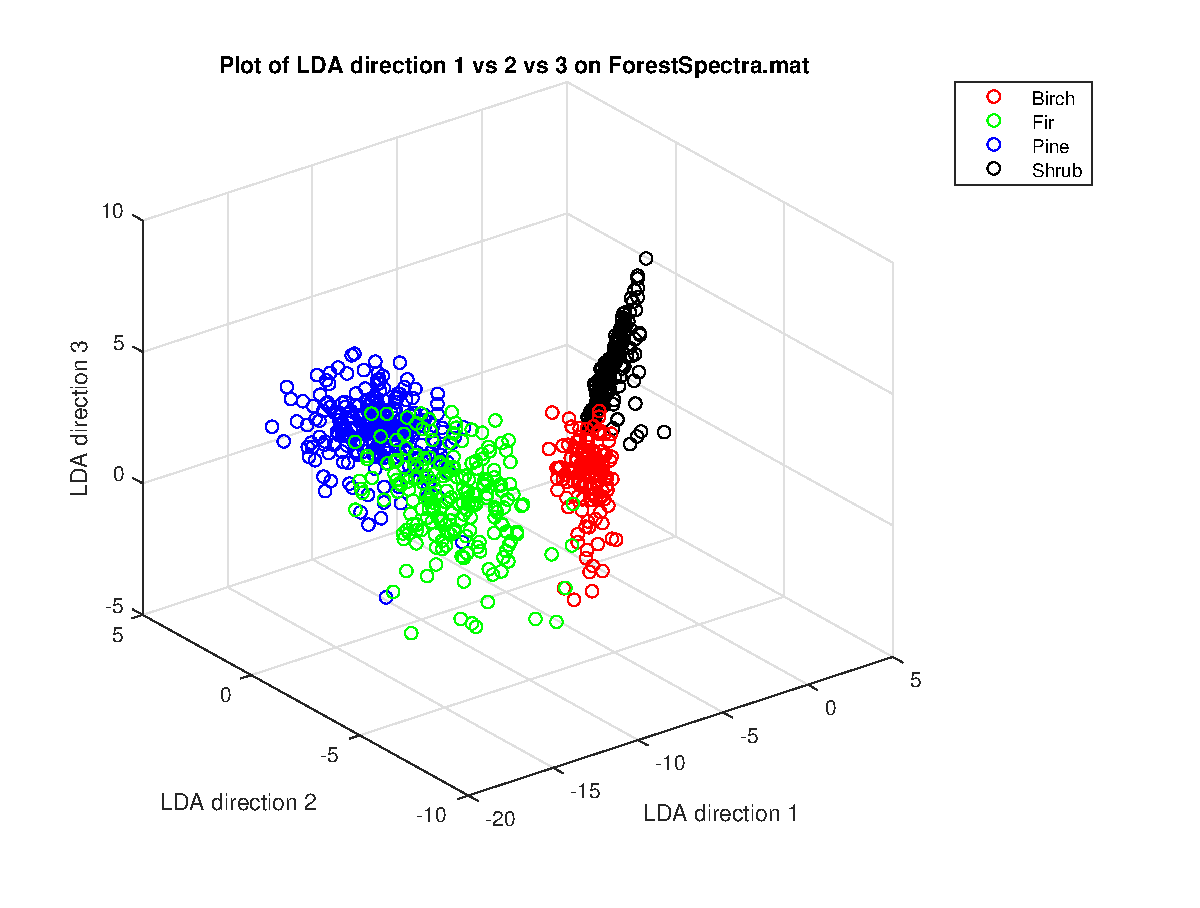
\includegraphics[width=15cm, height=6.5cm]{Q3_3directions}
    }
    \caption{\label{fig:my figure} LDA Clustering of 'ForestSpectra.mat' along first 3 LDA directions }
\end{figure}

\begin{figure}[H]
    \centerline
    {
    \includegraphics[width=15cm, height=6.5cm]{Q3_SF}
    }
    \caption{\label{fig:my figure} Success Frequency as a function of number of LDA Directions for ForestSpectraTest data.  Note that the success frequency plateaus once we have 4 LDA directions.}
\end{figure}

\subsection*{Analysis}
Since we have 4 clusters, it makes sense that the maximum value of the success frequency occurs when the number of LDA directions is 4.  


\end{document}
